
\documentclass[11pt,compress,t,notes=noshow]{beamer}

\usepackage[english]{babel}
\usepackage{dsfont}
\newcommand\bmmax{2}
\usepackage{bm}
\usepackage{bbm}
\usepackage{verbatim}
\usepackage{amsmath}
\usepackage{amsfonts}
\usepackage{csquotes}
\usepackage{multirow}
\usepackage{longtable}
\usepackage{enumerate}
\usepackage[absolute,overlay]{textpos}
\usepackage{psfrag}
\usepackage{algorithm}
\usepackage{algorithmicx}
\usepackage{algpseudocode}
\usepackage{eqnarray}
\usepackage{multimedia}
\usepackage{media9}
\usepackage{arydshln}
\usepackage{tabularx}
\usepackage{placeins}
\usepackage{tikz}
\usepackage{setspace}
\usepackage{wrapfig}
\usepackage{tcolorbox}
\usepackage[export]{adjustbox}
\usepackage{siunitx}
\usetikzlibrary{shapes,arrows,automata,positioning,calc}
\tikzset{
  %Define standard arrow tip
  >=stealth',
  %Define style for boxes
  punkt/.style={
    rectangle,
    rounded corners,
    draw=black, very thick,
    text width=6.5em,
    minimum height=2em,
    text centered},
  % Define arrow style
  pil/.style={
    ->,
    thick,
    shorten <=2pt,
    shorten >=2pt,}
}
\usepackage{subfig}

%new environments

\newenvironment{vbframe}  %frame with breaks and verbatim
{
 \begin{frame}[containsverbatim,allowframebreaks]
}
{
\end{frame}
}

\newenvironment{vframe}  %frame with verbatim without breaks (to avoid numbering one slided frames)
{
 \begin{frame}[containsverbatim]
}
{
\end{frame}
}

\newenvironment{blocki}[1]   % itemize block
{
 \begin{block}{#1}\begin{itemize}
}
{
\end{itemize}\end{block}
}

\newenvironment{fragileframe}[2]{  %fragile frame with framebreaks
\begin{frame}[allowframebreaks, fragile, environment = fragileframe]
\frametitle{#1}
#2}
{\end{frame}}


\newcommand{\myframe}[2]{  %short for frame with framebreaks
\begin{frame}[allowframebreaks]
\frametitle{#1}
#2
\end{frame}}

\newcommand{\remark}[1]{
  \textbf{Remark:} #1
}

%%%%%%%%%%%%%%%%%%%%%%%%%%%%%%%%%%%%%%%%%%%%%%%%%%%%%%%%%%%%%%%%%%%%%%%%%%%%%%%

% basic latex stuff
\newcommand{\pkg}[1]{{\fontseries{b}\selectfont #1}} %fontstyle for R packages
\newcommand{\lz}{\vspace{0.5cm}} %vertical space
\newcommand{\dlz}{\vspace{1cm}} %double vertical space
\newcommand{\oneliner}[1] % Oneliner for important statements
{\begin{block}{}\begin{center}\begin{Large}#1\end{Large}\end{center}\end{block}}


%\usetheme{lmu-lecture}
\usepackage{../style/lmu-lecture}

\let\code=\texttt
\let\proglang=\textsf

\setkeys{Gin}{width=0.9\textwidth}


\title{Deep Learning}
\author{Mina Rezaei}
\institute{Department of Statistics -- LMU Munich}
\date{Winter Semester 2021}

\setbeamertemplate{frametitle}{\expandafter\uppercase\expandafter\insertframetitle}

%\begin{document}
%\sloppy
%\end{document}


\input{../../latex-math/basic-math}
\input{../../latex-math/basic-ml}
\input{../../latex-math/ml-nn}

\begin{document}

\lecturechapter{6}{Modern Convolutional Neural Networks}
\lecture{Deeplearning}
%%%%%%%%%%%%%%%%%%%%%%%%%%%%%%%%%%%%%%%%%%%%%%%%%%%%%%%%%%%%%%%%%%

\begin{frame}
\frametitle{Lecture outline}
\tableofcontents
\end{frame}

%%%%%%%%%%%%%%%%%%%%%%%%%%%%%%%%%%%%%%%%%%%%%%%%%%%%%%%%%%%%%%%%%%

\section{From LeNet to AlexNet}

\begin{vbframe}{LeNet Architecture}
  \begin{itemize}
    \item Pioneering work on CNNs by Yann Lecun in 1998. 
    \item Applied on the MNIST dataset for automated handwritten digit recognition.
    \item Consists of convolutional, "subsampling" and dense layers.
    \item Complexity and depth of the net was mainly restricted by limited computational power back in the days.
  \end{itemize}
  \begin{figure}
  \centering
    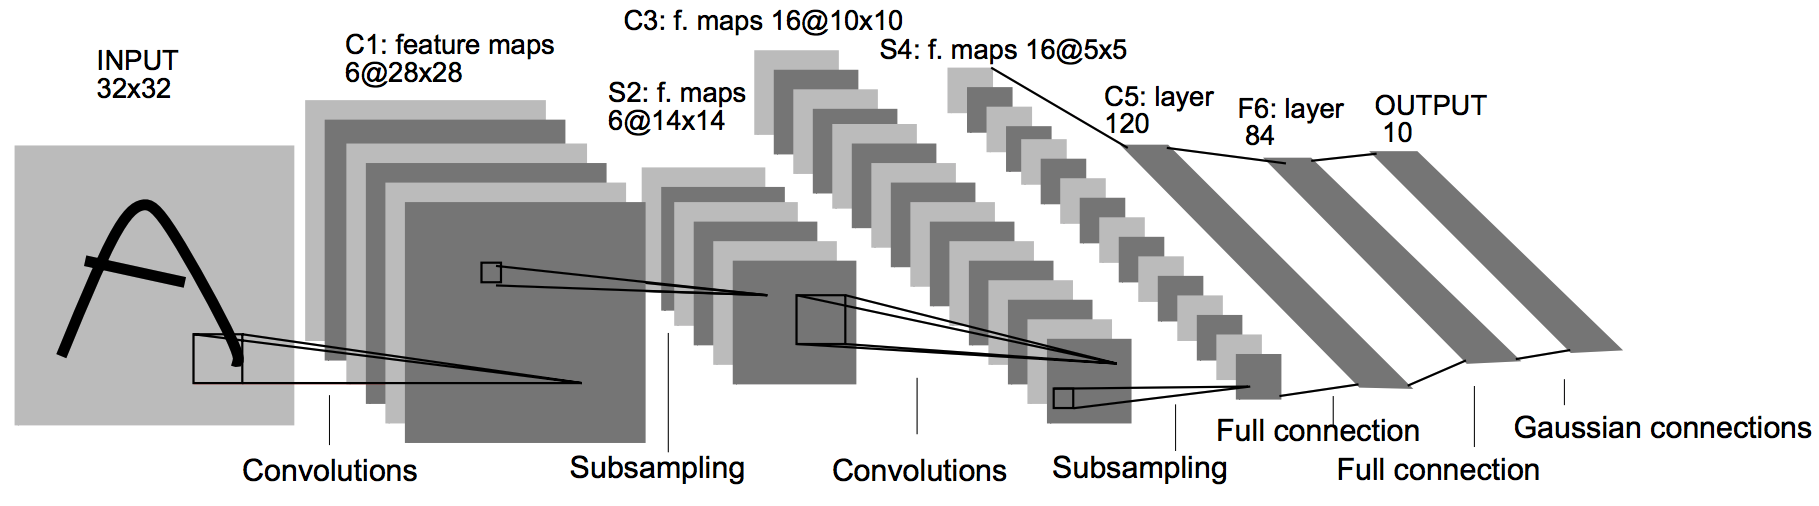
\includegraphics[width=9cm]{plots/architectures/lenet.png}
    \caption{LeNet architecture: two conv layers with subsampling, followed by dense layers and a 'Gaussian connections' layer.}
  \end{figure}
  \framebreak
  \begin{itemize}
    \item A neuron in a subsampling layer looks at a $2 \times 2$ region of a feature map, sums the four values, multiplies it by a trainable coefficient, adds a trainable bias and then applies a sigmoid activation.
    \item A stride of 2 ensures that the size of the feature map reduces by about a half.
    \item The 'Gaussian connections' layer has a neuron for each possible class. 
    \item The output of each neuron in this layer is the (squared) Euclidean distance between the activations from the previous layer and the weights of the neuron.
  \end{itemize}   
\end{vbframe}


\begin{vbframe}{AlexNet}
  \begin{itemize}
    \item AlexNet, which employed an 8-layer CNN, won the ImageNet Large Scale Visual Recognition (LSVR) Challenge 2012 by a phenomenally large margin.
    \item The network trained in parallel on two small GPUs, using two streams of convolutions which are partly interconnected.
    \item The architectures of AlexNet and LeNet are very similar, but there are also significant differences: 
       \begin{itemize}
          \item First, AlexNet is deeper than the comparatively small LeNet5. AlexNet consists of eight layers: five convolutional layers, two fully-connected hidden layers, and one fully-connected output layer. 
          \item Second, AlexNet used the ReLU instead of the sigmoid as its activation function. 
       \end{itemize}
  \end{itemize}
    \begin{figure}
        \centering
        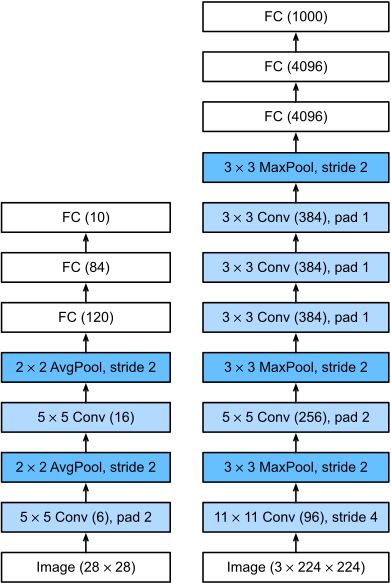
\includegraphics[width=4.5cm]{plots/moderncnn/alexnet.png}
        \caption{From LeNet (left) to AlexNet (right).}
    \end{figure}
    
        \begin{figure}
        \centering
        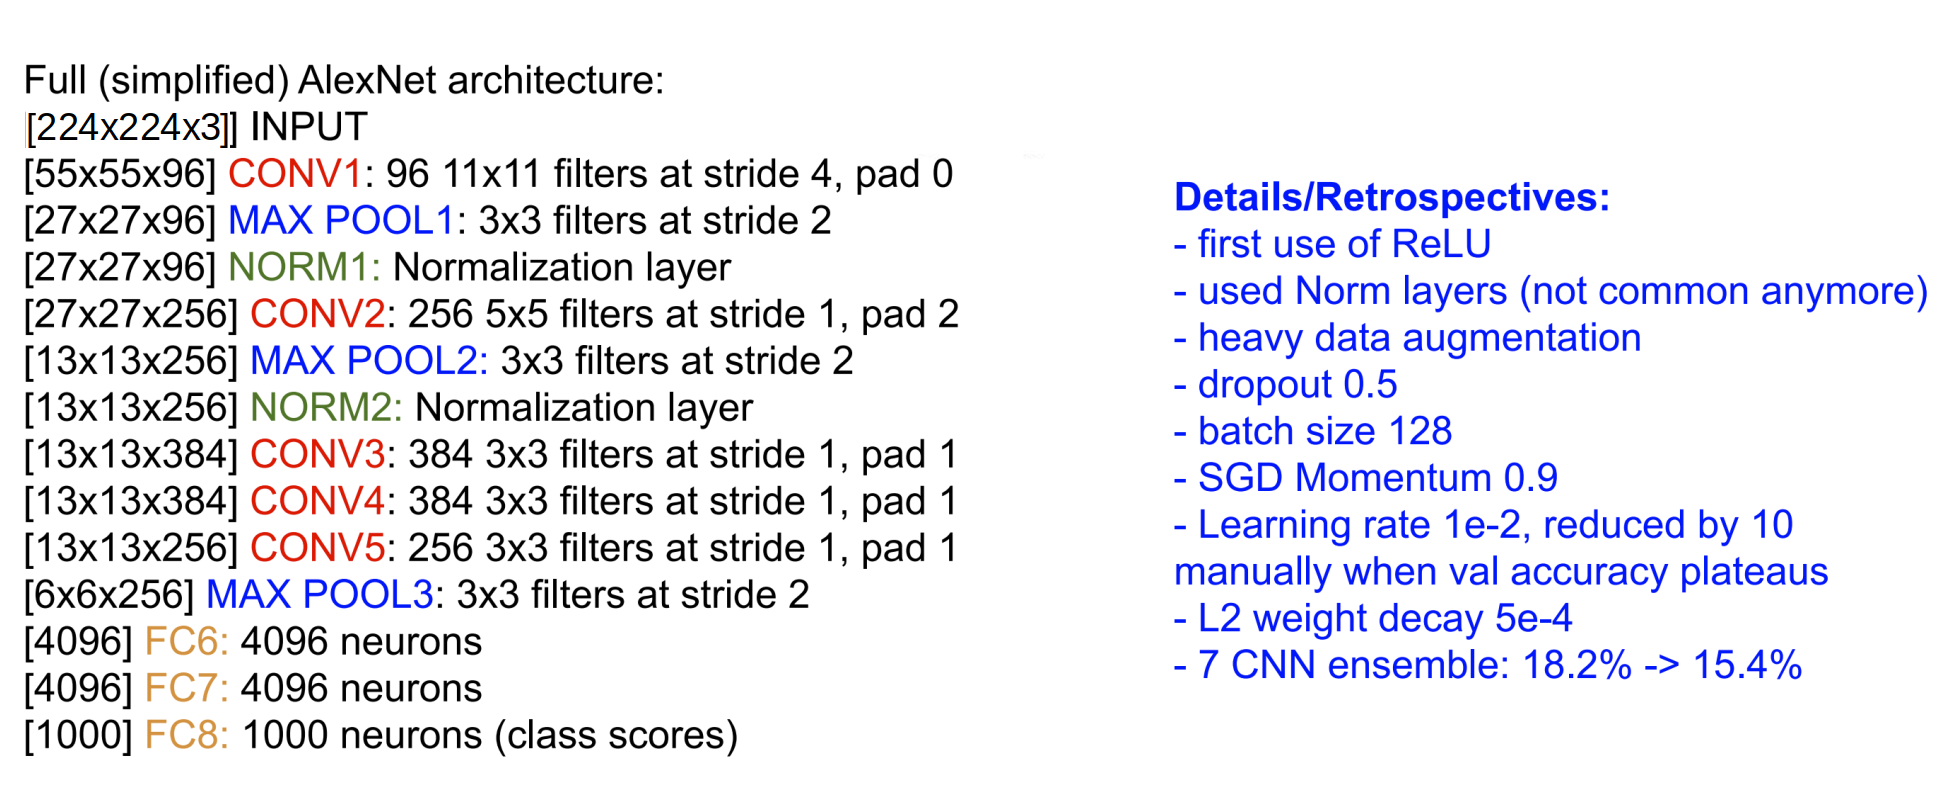
\includegraphics[width=11cm]{plots/moderncnn/alexnet_detail.png}
                    \tiny{\\ credit : Stanford Cs231n}
        \caption{Implementation detail by AlexNet.}
    \end{figure}
    
\end{vbframe}

%%%%%%%%%%%%%%%%%%%%%%%%%%%%%%%%%%%%%%%%%%%%%%%%%%%%%%%%%%%%%%%%%%

\begin{vbframe}{ImageNet Large Scale Visual Recognition Challenge (ILSVRC) winners}

    \begin{figure}
        \centering
        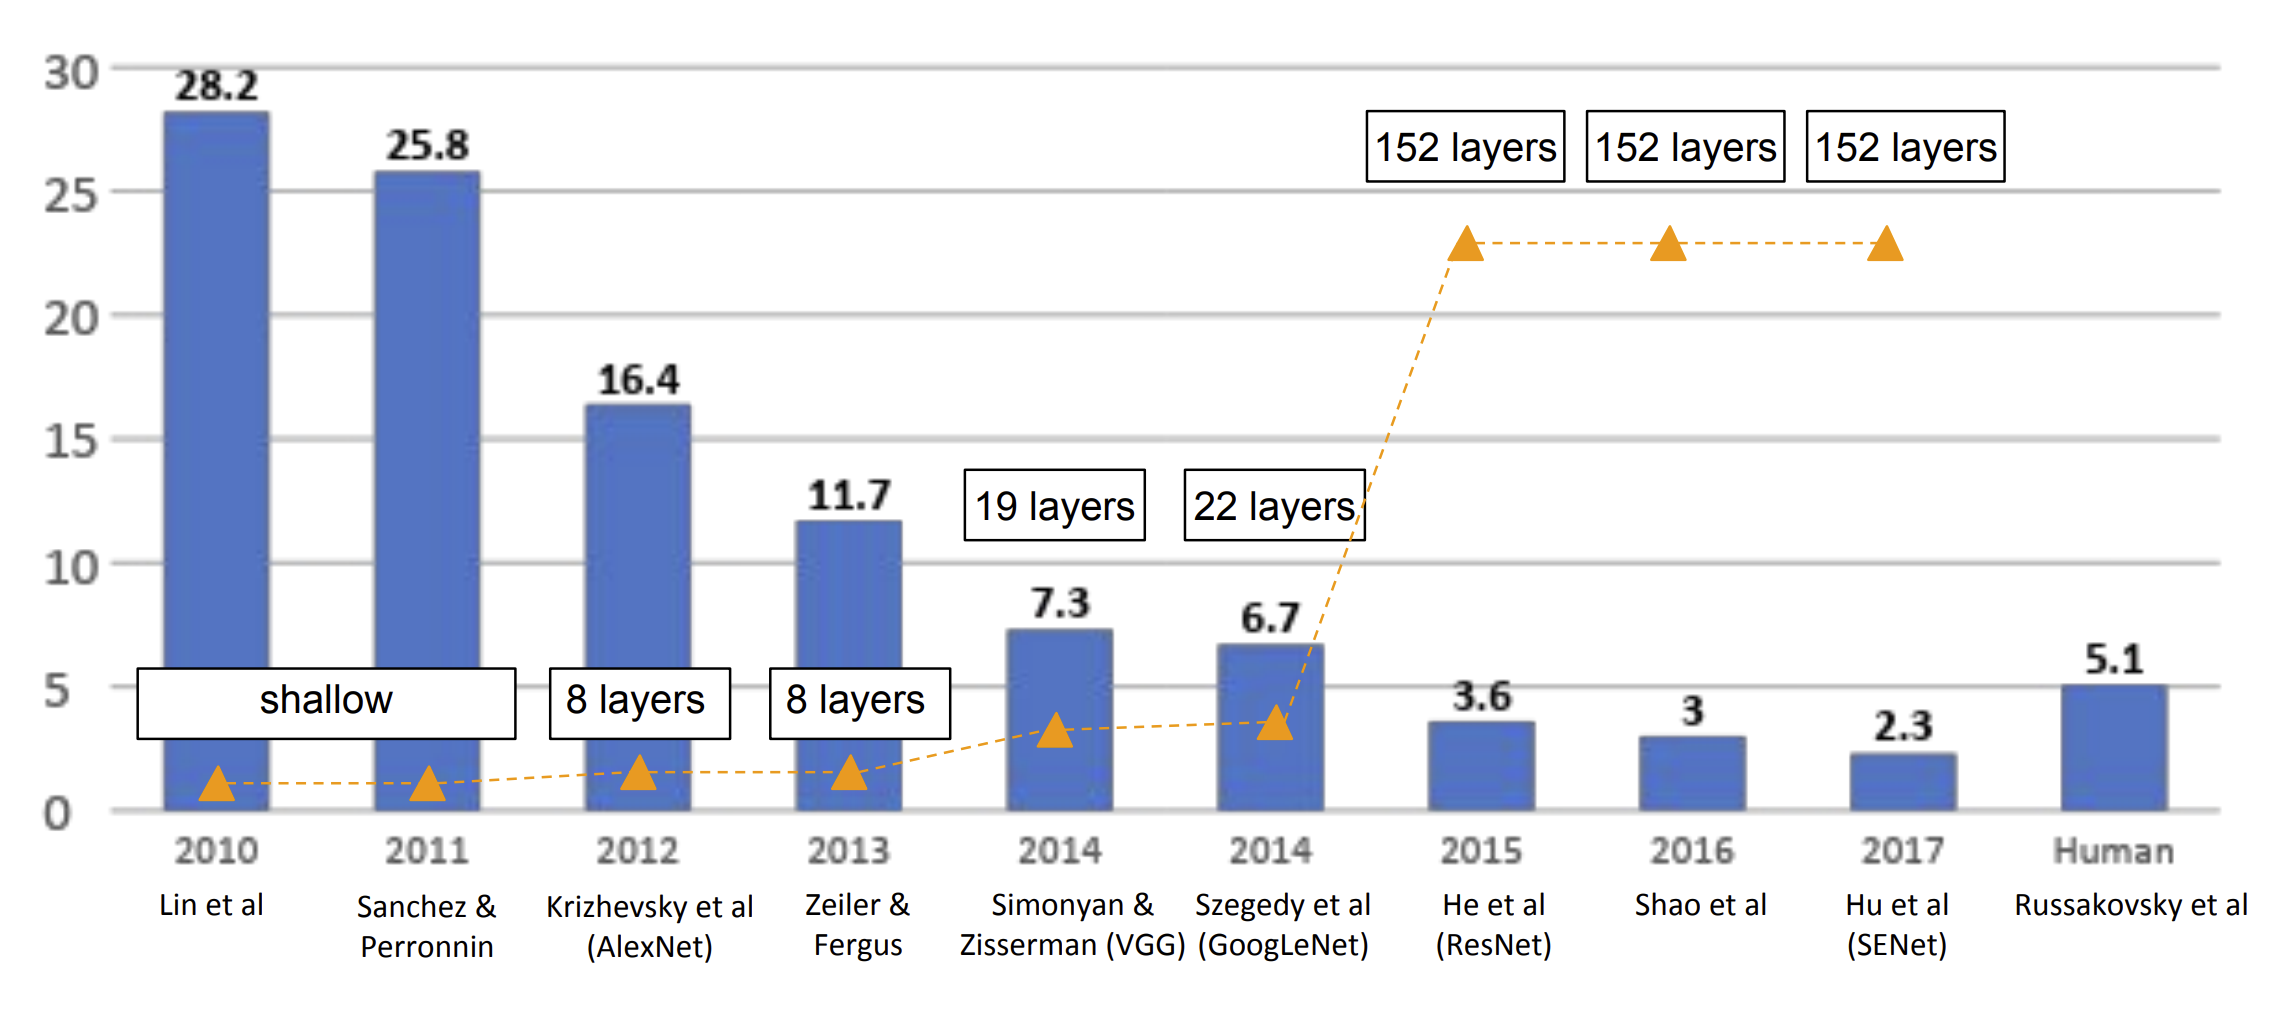
\includegraphics[width=10cm]{plots/moderncnn/imagenet.png}
            \tiny{\\ credit : Stanford Cs231n}
        \caption{ILSVRC Compitions winners.}
    \end{figure}
    
\end{vbframe}

\begin{vbframe}{ZFNet}

It has similar architecture of AlexNet but:
       \begin{itemize}
          \item CONV1: change from ($11 \times 11$ stride 4) to (7 x 7 stride 2)
          \item CONV3,4,5: instead of 384, 384, 256 filters use 512, 1024, 512
          \item ImageNet top 5 error: 16.4\% to 11.7\%
       \end{itemize}

\end{vbframe}
%%%%%%%%%%%%%%%%%%%%%%%%%%%%%%%%%%%%%%%%%%%%%%%%%%%%%%%%%%%%%%%%%%
    

\section{Networks Using Blocks (VGG)}

\begin{vbframe}{VGG Blocks}
  \begin{itemize}
    \item The block composed of convolutions with $3 \times 3$  kernels with padding of 1 (keeping height and width) and $2 \times 2$  max pooling with stride of 2 (having the resolution after each block).
    \item The use of blocks leads to very compact representations of the network definition. 
    \item It allows for efficient design of complex networks.
  \end{itemize}
  
    \begin{figure}
  \centering
    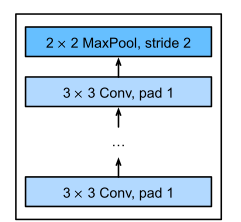
\includegraphics[width=3cm]{plots/moderncnn/vggblock.png}
    \tiny{\\ credit : D2DL}
    \caption{VGG block.}
  \end{figure}
  
\end{vbframe}



\begin{vbframe}{VGG Network}
  \begin{itemize}
    \item Architecture introduced by Simonyan and Zisserman, 2014 as \enquote{Very Deep Convolutional Network}.
    \item A deeper variant of the AlexNet.
    \item Basic idea is to have small filters and Deeper networks
    \item Mainly uses many cnn layers with a small kernel size $3 \times 3$.
    \item Stack of three $3 \times 3$ cnn (stride 1) layers has same effective receptive field as one $7 \times 7$ conv layer. But It's deeper, more non-linearities, and fewer parameters
    \item Performed very well in the ImageNet Challenge in 2014.
    \item Exists in a small version (VGG16) with a total of 16 layers (13 cnn layers and 3 fc layers) and 5 VGG blocks while a larger version (VGG19) with 19 layers (16 cnn layers and 3 fc layers) and 6 VGG blocks.
  \end{itemize}
  
\framebreak

  \begin{figure}
  \centering
    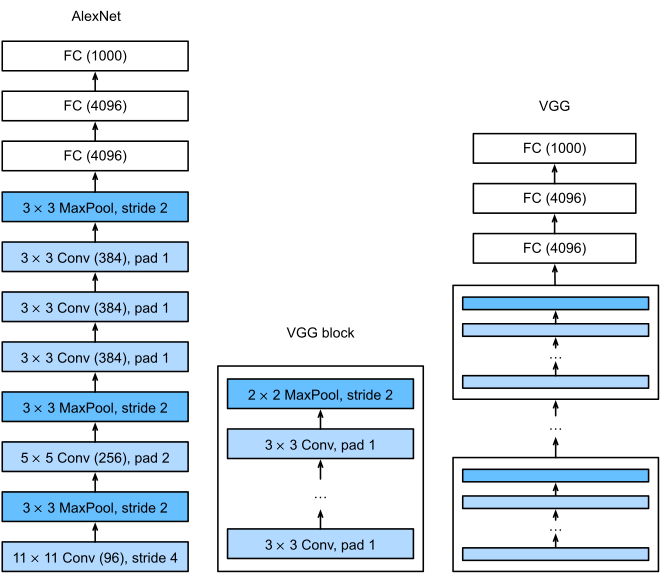
\includegraphics[width=7cm]{plots/moderncnn/vgg.png}
    \tiny{\\ credit : D2DL}
    \caption{From AlexNet to VGG that is designed from building blocks.}
  \end{figure}
  
          \begin{figure}
        \centering
        \includegraphics[width=11cm]{plots/moderncnn/VGG_detail.png}
                    \tiny{\\ credit : Stanford Cs231n}
        \caption{Computational complexity by VGG network.}
    \end{figure}

\end{vbframe}


%%%%%%%%%%%%%%%%%%%%%%%%%%%%%%%%%%%%%%%%%%%%%%%%%%%%%%%%%%%%%%%%%%
\section{Network in Network (NiN)}


\begin{vbframe}{NiN Blocks}
  \begin{itemize}
    \item The idea behind NiN is to apply a fully-connected layer at each pixel location (for each height and width). If we tie the weights across each spatial location, we could think of this as a $1 \times 1$ convolutional layer.
    \item The NiN block consists of one convolutional layer followed by two $1 \times 1$  convolutional layers that act as per-pixel fully-connected layers with ReLU activations.
    \item The convolution window shape of the first layer is typically set by the user. The subsequent window shapes are fixed to $1 \times 1$.
  \end{itemize}
  \begin{figure}
  \centering
    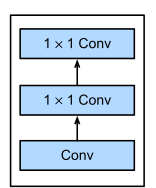
\includegraphics[width=2cm]{plots/moderncnn/ninblock.png}
    \tiny{\\ credit : D2DL}
    \caption{NiN block.}
  \end{figure}

\end{vbframe}


\begin{vbframe}{Global average pooling}
    \begin{itemize}
        \item Problem setting: tackle overfitting in the final fully connected layer.
        \begin{itemize}
        \item Classic pooling removes spatial information and is mainly used for dimension and parameter reduction.
        \item The elements of the final feature maps are connected to the output layer via a dense layer. This could require a huge number of weights increasing the danger of overfitting.
        \item Example: 256 feature maps of dim 100x100 connected to 10 output neurons lead to $256\times 10^5$ weights for the final dense layer.
        \end{itemize}
        

\framebreak 

        \item Solution: 
        \begin{itemize}
            \item Average each final feature map to the element of one global average pooling (GAP) vector.
            \item Example: 256 feature maps are now reduced to GAP-vector of length 256 yielding a final dense layer with 2560 weights.
        \end{itemize}
    \end{itemize}

    \begin{figure}
        \centering
        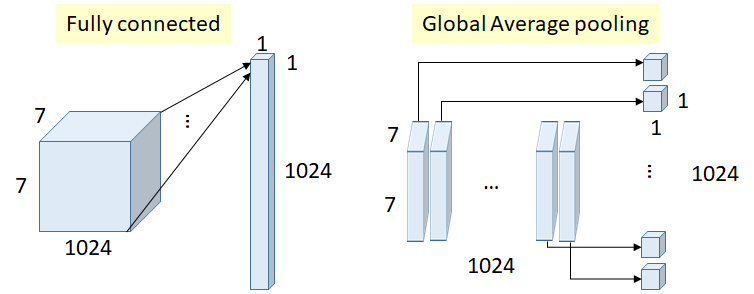
\includegraphics[width=8cm]{plots/moderncnn/GAP.png}
        \small{\caption{An Example of Fully Connected Layer VS Global Average Pooling Layer}}
    \end{figure}

\framebreak

    \begin{itemize}
        \item GAP preserves whole information from the single feature maps whilst decreasing the dimension.
        \item Mitigates the possibly \textbf{destructive} effect of pooling.
        \item Each element of the GAP output represents the activation of a certain feature on the input data.
        \item Acts as an additional regularizer on the final fully connected layer.
    \end{itemize}

\end{vbframe}


\begin{vbframe}{Network in Network (NiN)}
  \begin{itemize}
    \item NiN uses blocks consisting of a convolutional layer and multiple $1 \times 1$ convolutional layers. This can be used within the convolutional stack to allow for more per-pixel nonlinearity.
    \item NiN removes the fully-connected layers and replaces them with global average pooling (i.e., summing over all locations) after reducing the number of channels to the desired number of outputs (e.g., 10 for Fashion-MNIST).
    \item Removing the fully-connected layers reduces overfitting. NiN has dramatically fewer parameters.
    \item The NiN design influenced many subsequent CNN designs.
  \end{itemize}
\framebreak
  \begin{figure}
  \centering
    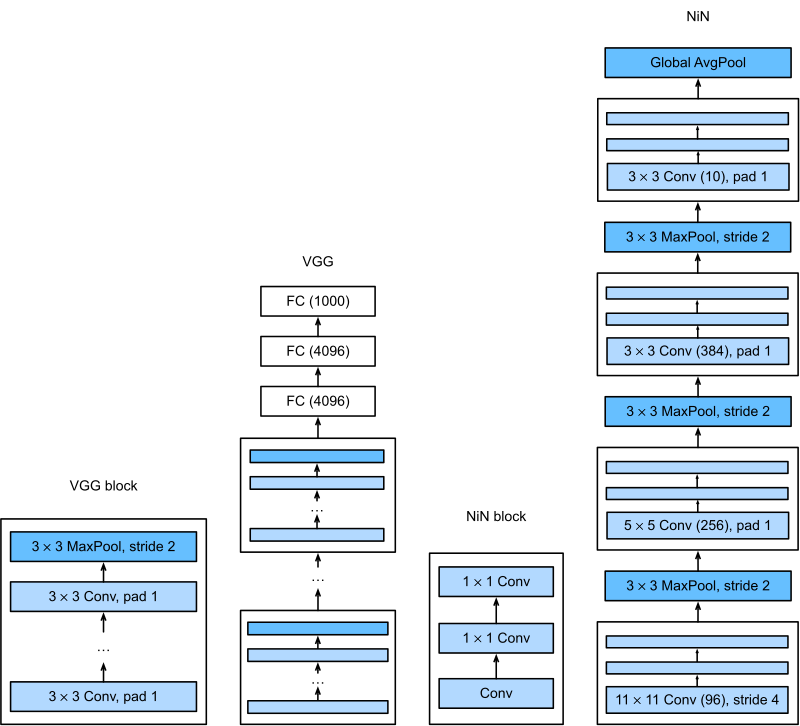
\includegraphics[width=7cm]{plots/moderncnn/nin.png}
    \tiny{\\ credit : D2DL}
    \caption{Comparing architectures of VGG and NiN, and their blocks.}
  \end{figure}

\end{vbframe}

%%%%%%%%%%%%%%%%%%%%%%%%%%%%%%%%%%%%%%%%%%%%%%%%%%%%%%%%%%%%%%%%%%
\section{Networks with Parallel Concatenations (GoogLeNet)}


\begin{vbframe}{Inception Block}
    \begin{itemize}
        \item Problem setting: how do we choose the kernel size in each layer? 
        \item This is often an arbitrary decision.
        \item Solution: offer the model kernels of different sizes in each layer through which it can propagate information and let it decide, which one to use to which extent.
        \item Side-effect: massive parameter reduction allowing for deeper architectures.
    \end{itemize}
    
      \begin{figure}
    \centering
      \scalebox{0.7}{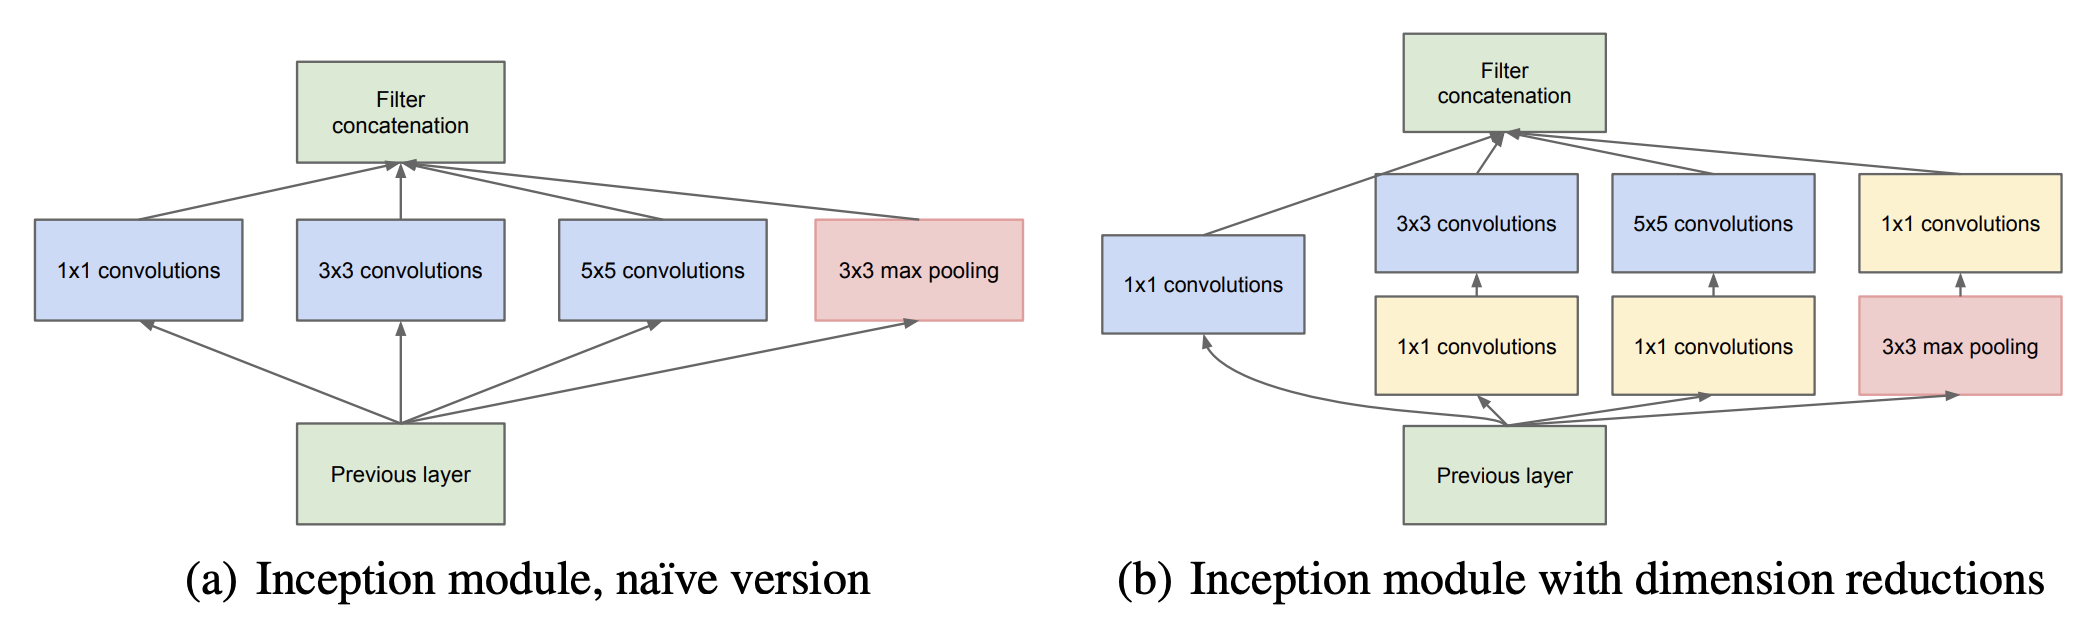
\includegraphics{plots/moderncnn/inception1.png}}
    \caption{Inception block.}
  \end{figure}
    
\end{vbframe}
         
         
\begin{vbframe}{Inception Block}
    \begin{itemize}
        \item The Inception block is equivalent to a subnetwork with four paths. 
        \item It extracts information in parallel through convolutional layers of different window shapes and max-pooling layers.  
        \item $1 \times 1$ convolutions reduce channel dimensionality on a per-pixel level. Max-pooling is used as it is ought to increase the robustness of the feature maps. The kernels are padded accordingly to yield feature maps of equal dimensions..
    \end{itemize}
    
    
  \begin{figure}
    \centering
      \scalebox{0.75}{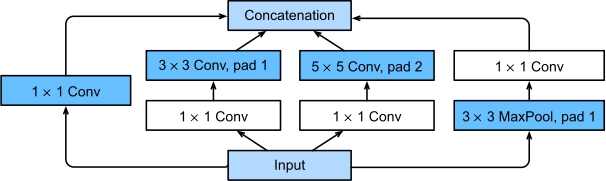
\includegraphics{plots/moderncnn/inception.png}}
    \caption{Inception block with dimention reduction.}
  \end{figure}
\end{vbframe}



\begin{vbframe}{GoogLeNet Architecture}
    \begin{itemize}
        \item GoogLeNet connects multiple well-designed Inception blocks with other layers in series. 
        \item The ratio of the number of channels assigned in the Inception block is obtained through a large number of experiments on the ImageNet dataset.
        \item GoogLeNet, as well as its succeeding versions, was one of the most efficient models on ImageNet, providing similar test accuracy with lower computational complexity.
    \end{itemize}
    
\framebreak

\begin{figure}
  \centering
    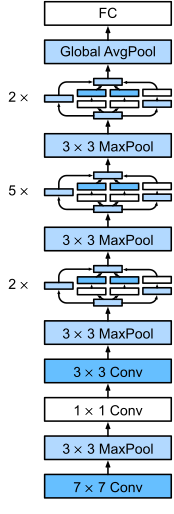
\includegraphics[width=2cm]{plots/moderncnn/inception-full.png}
    \tiny{\\ credit : D2DL}
    \caption{The GoogLeNet architecture.}
\end{figure}
    
    
\begin{figure}
  \centering
    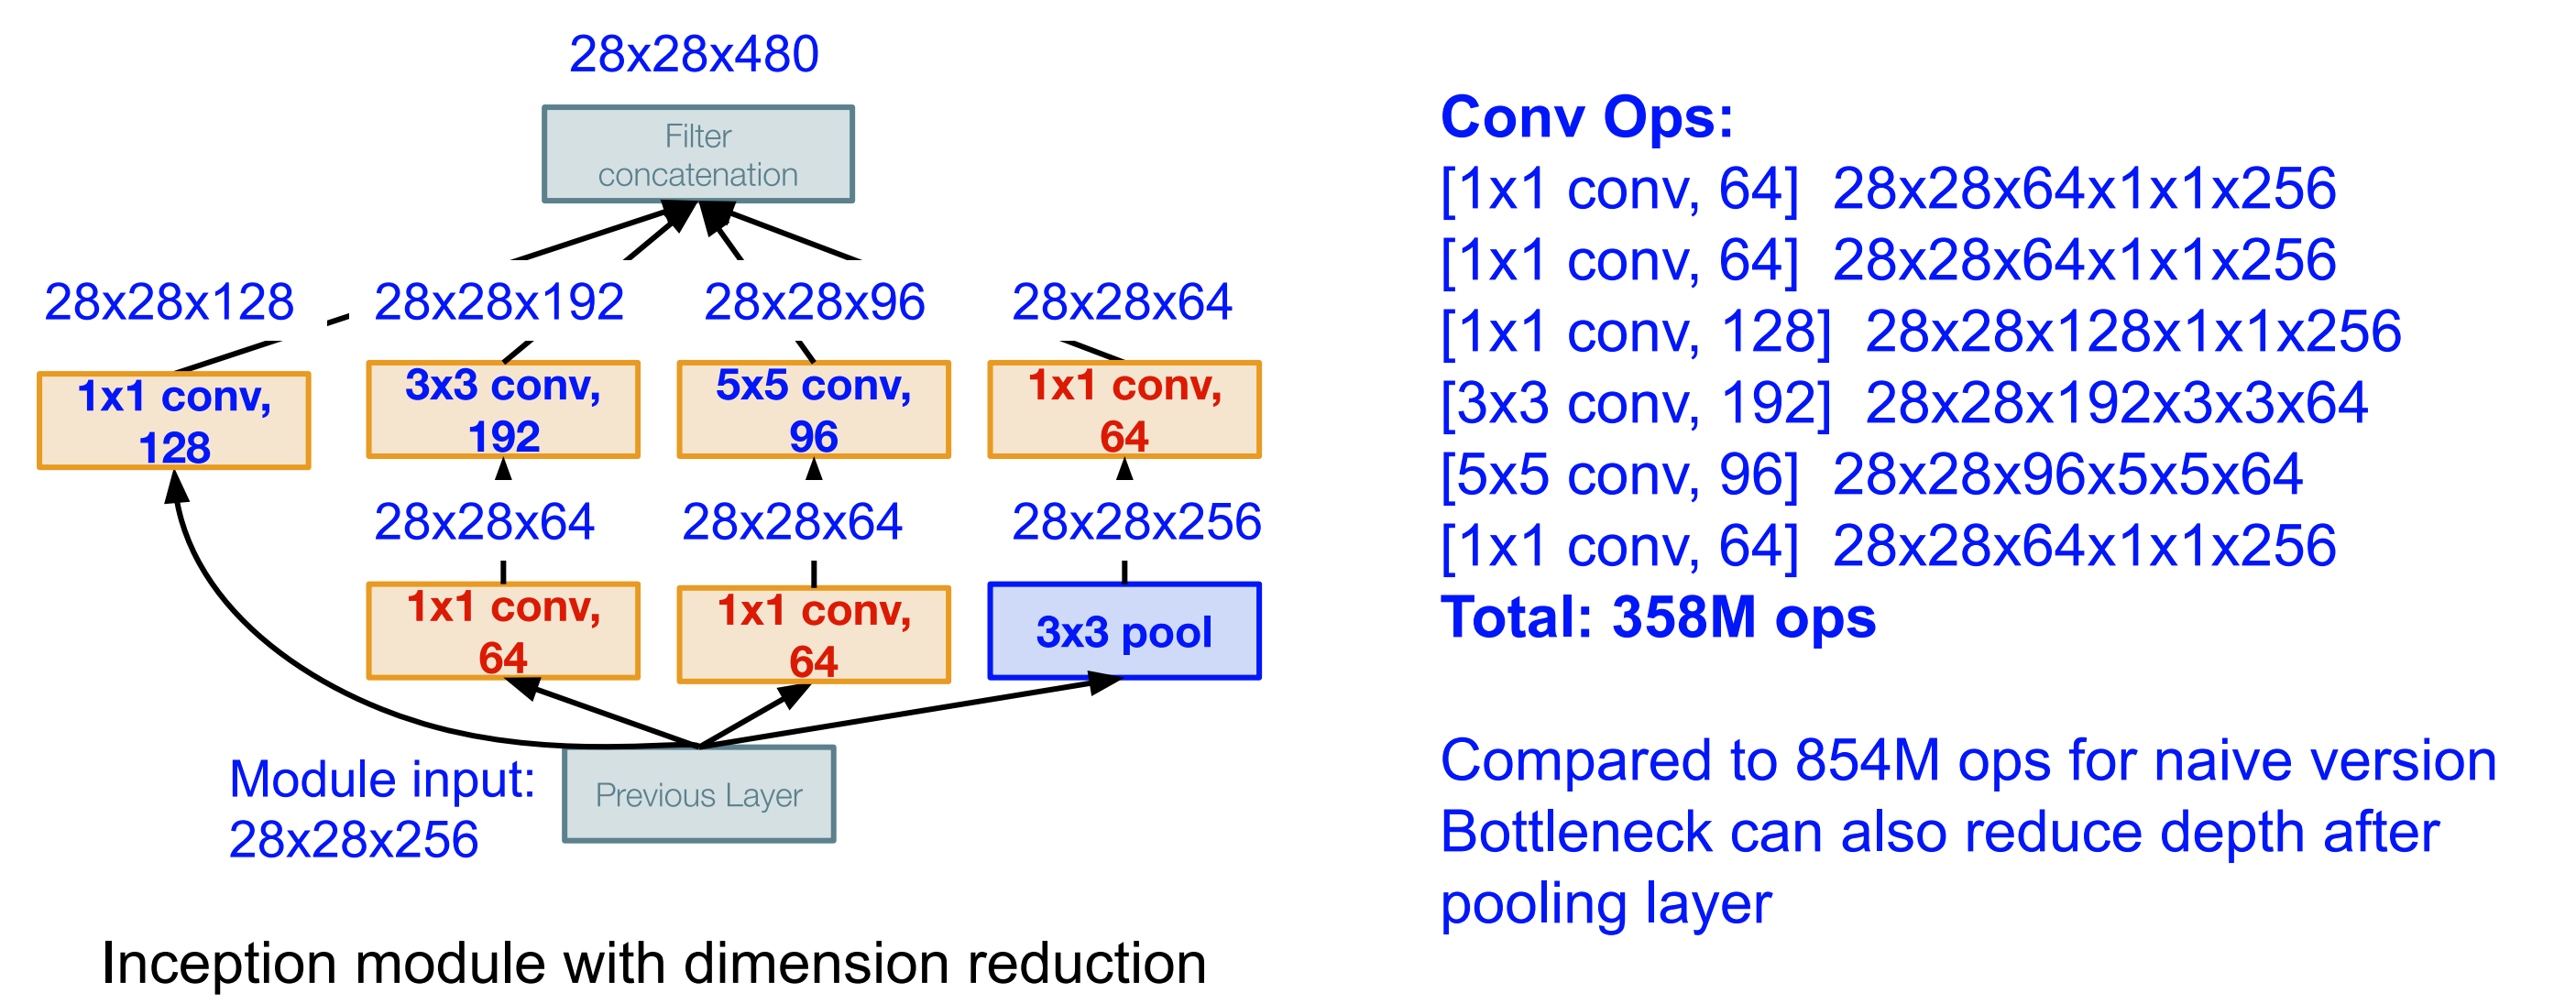
\includegraphics[width=11cm]{plots/moderncnn/inception_detail.png}
    \tiny{\\ credit : Stanford cs231n}
    \caption{Computational complexity by Inceptation module }
\end{figure}
    
\end{vbframe}

%%%%%%%%%%%%%%%%%%%%%%%%%%%%%%%%%%%%%%%%%%%%%%%%%%%%%%%%%%%%%%%%%%

\section{Residual Networks (ResNet)}

%\subsection{Residual Block}

\begin{vbframe}{Residual Block (Skip connections)}

What happens when we continue stacking deeper layers on a $"$plain$"$ convolutional
neural network?
      \begin{figure}
    \centering
      \scalebox{0.8}{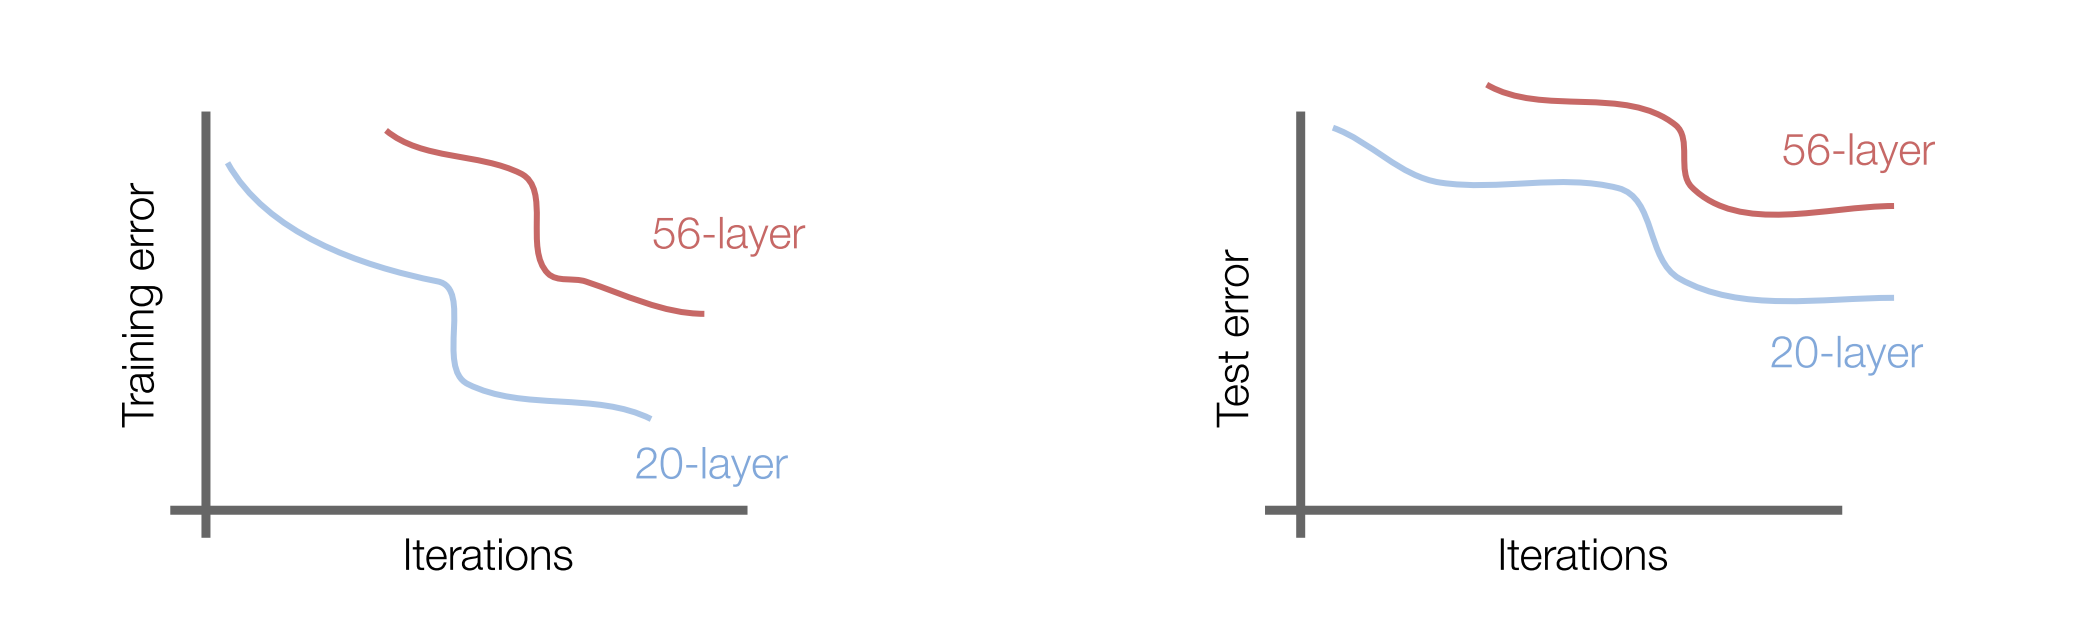
\includegraphics{plots/moderncnn/resnet0.png}}
    \tiny{\\ credit : Stanford cs231n}
    \tiny{\\56-layer model performs worse on both training and test error! The deeper model performs worse, but it's not caused by overfitting!}
  \end{figure}
    

    \begin{itemize}
        \item Fact: Deep models have more representation power (more parameters) than shallower models.
        \item Hypothesis: the problem is an optimization problem, \textbf{deeper models are harder to optimize}
        \item Problem setting: theoretically, we could build infinitely deep architectures as the net should learn to pick the beneficial layers and skip those that do not improve the performance automatically.
        \item But: this skipping would imply learning an identity mapping $\xv = \mathcal{F}(\xv)$. It is very hard for a neural net to learn such a 1:1 mapping through the many non-linear activations in the architecture.
        \item Solution: offer the model explicitly the opportunity to skip certain layers if they are not useful.
        \item Introduced in \textit{He et. al , 2015} and motivated by the observation that stacking evermore layers increases the test- as well as the train-error ($\neq$ overfitting).
    \end{itemize}
    
\framebreak
 
 \begin{figure}
  \centering
    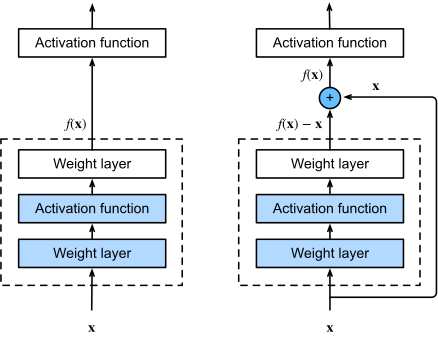
\includegraphics[width=6cm]{plots/moderncnn/residual-block.png}
    \tiny{\\ credit : D2DL}
    \caption{A regular block (left) and a residual block (right).}
  \end{figure}

  \begin{figure}
  \centering
    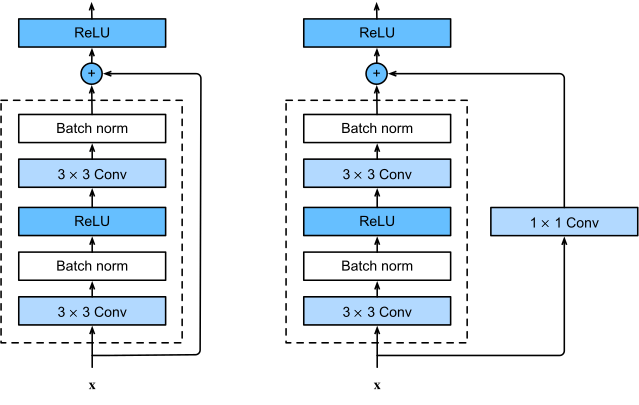
\includegraphics[width=6cm]{plots/moderncnn/resnet-block.png}
    \tiny{\\ credit : D2DL}
    \caption{ResNet block with and without $1 \times 1$ convolution.The information flows through two layers and the identity function. Both streams of information are then element-wise summed and jointly activated.}
  \end{figure}

\framebreak
    \begin{itemize}
        \item Let $\mathcal{H}(\xv)$ be the optimal underlying mapping that should be learned by (parts of) the net.
        \item $\xv$ is the input in layer $l$ (can be raw data input or the output of a previous layer).
        \item $\mathcal{H}(\xv)$ is the output from layer $l$.
        \item Instead of fitting $\mathcal{H}(\xv)$, the net is ought to learn the residual mapping $\mathcal{F}(\xv):=\mathcal{H}(\xv)-\xv$ whilst $\xv$ is added via the identity mapping.
        \item Thus, $\mathcal{H}(\xv) = \mathcal{F}(\xv) + \xv$, as formulated on the previous slide.
        \item The model should only learn the \textbf{residual mapping} $\mathcal{F}(\xv)$ 
        \item Thus, the procedure is also referred to as \textbf{Residual Learning}.
    \end{itemize}
    
\framebreak


    \begin{itemize}
        \item The element-wise addition of the learned residuals $\mathcal{F}(\xv)$ and the identity-mapped data $\xv$ requires both to have the same dimensions.
        \item To allow for downsampling within $\mathcal{F}(\xv)$ (via pooling or valid-padded convolutions), the authors introduce a linear projection layer $W_s$ .
        \item $W_s$ ensures that $\xv$ is brought to the same dimensionality as $\mathcal{F}(\xv)$ such that:
        $$
            y = \mathcal{F}(\xv) + W_s\xv,
        $$
        \item $y$ is the output of the skip module and $W_s$ represents the weight matrix of the linear projection (\# rows of $W_s$ = dimensionality of $\mathcal{F}(\xv)$).
        \item This idea applies to fully connected layers as well as to convolutional layers.
    \end{itemize}
\end{vbframe}


\framebreak

\begin{vbframe}{ResNet Architecture}
    \begin{itemize}
        \item The residual mapping can learn the identity function more easily, such as pushing parameters in the weight layer to zero.
        \item We can train an effective deep neural network by having residual blocks.
        \item Inputs can forward propagate faster through the residual connections across layers.
        \item ResNet had a major influence on the design of subsequent deep neural networks, both for convolutional and sequential nature.
    \end{itemize}
    
     \begin{figure}
  \centering
    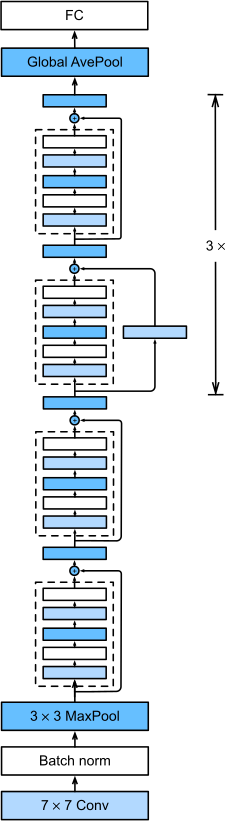
\includegraphics[width=2cm]{plots/moderncnn/resnet18.png}
    \tiny{\\ credit : D2DL}
    \caption{The ResNet-18 architecture.}
  \end{figure}
  
 \end{vbframe}

%%%%%%%%%%%%%%%%%%%%%%%%%%%%%%%%%%%%%%%%%%%%%%%%%%%%%%%%%%%%%%%%%%
\section{Densely Connected Networks (DenseNet)}

%\subsection{Dense Blocks}
\begin{vbframe}{From ResNet to DenseNet}
    \begin{itemize}
        \item ResNet significantly changed the view of how to parametrize the functions in deep networks. 
        \item DenseNet (dense convolutional network) is to some extent the logical extension of this [Huang et al., 2017]. 
        \item Dense blocks where each layer is connected to every other layer in feedforward fashion.
        \item Alleviates vanishing gradient, strengthens feature propagation, encourages feature reuse.
        \item To understand how to arrive at it, let us take a small detour to mathematics: 
        \begin{itemize}
             \item Recall the Taylor expansion for functions. For the point  $x=0$  it can be written as: $f(x) = f(0) + f'(0) x + \frac{f''(0)}{2!}  x^2 + \frac{f'''(0)}{3!}  x^3 + \ldots.$
             \item The key point is that it decomposes a function into increasingly higher order terms. In a similar vein, ResNet decomposes functions into : $f(\mathbf{x}) = \mathbf{x} + g(\mathbf{x}).$
             \item That is, ResNet decomposes  f  into a simple linear term and a more complex nonlinear one. What if we want to capture (not necessarily add) information beyond two terms? One solution was DenseNet [Huang et al., 2017].
        \end{itemize}
    \end{itemize}
    
     \begin{figure}
  \centering
    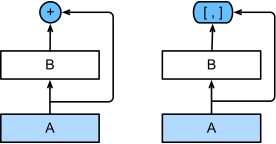
\includegraphics[width=4cm]{plots/moderncnn/densenet-block.png}
    \tiny{\\ credit : D2DL}
    \caption{ DensNet Block.}
  \end{figure}
  
 % \subsection{DenseNet Model}
  
  As shown in previous Figure, the key difference between ResNet and DenseNet is that in the latter case outputs are concatenated (denoted by  $[,]$ ) rather than added. As a result, we perform a mapping from  $x$  to its values after applying an increasingly complex sequence of functions:
  \newline
  \newline
$\mathbf{x} \to \left[ \mathbf{x}, f_1(\mathbf{x}), f_2([\mathbf{x}, f_1(\mathbf{x})]), f_3([\mathbf{x}, f_1(\mathbf{x}), f_2([\mathbf{x}, f_1(\mathbf{x})])]), \ldots\right].$
\newline
\newline
In the end, all these functions are combined in MLP to reduce the number of features again. In terms of implementation this is quite simple: rather than adding terms, we concatenate them. 
\newline
The name DenseNet arises from the fact that the dependency graph between variables becomes quite dense. The last layer of such a chain is densely connected to all previous layers. 
  \begin{figure}
    \centering
    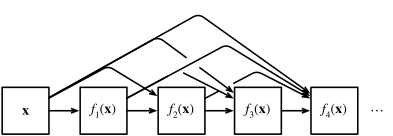
\includegraphics[width=4cm]{plots/moderncnn/densenet.png}
    \tiny{\\ credit : D2DL}
    \caption{The DensNet architecture.}
  \end{figure}
  
 \end{vbframe}



%%%%%%%%%%%%%%%%%%%%%%%%%%%%%%%%%%%%%%%%%%%%%%%%%%%%%%%%%%%%%%%%%%
%%%%%%%%%%%%%%%%%%%%%%%%%%%%%%%%%%%%%%%%%%%%%%%%%%%%%%%%%%%%%%%%%%

%%%%%%%%%%%%%%%%%%%%%%%%%%%%%%%%%%%%%%%%%%%%%%%%%%%%%%%%%%%%%%%%%%
%%%%%%%%%%%%%%%%%%          REFERENCES          %%%%%%%%%%%%%%%%%%
%%%%%%%%%%%%%%%%%%%%%%%%%%%%%%%%%%%%%%%%%%%%%%%%%%%%%%%%%%%%%%%%%%
\begin{vbframe}
\frametitle{References}
\footnotesize{
\begin{thebibliography}{99}

% \bibitem[Ronneberger et al., 2015]{12} Olaf Ronneberger, Philipp Fischer, Thomas Brox (2015)
% \newblock U-Net: Convolutional Networks for Biomedical Image Segmentation
% \newblock \emph{\url{http://arxiv.org/abs/1505.04597}}
% %%%%%%%%%%%%%%%%%%%%%%%%%%%%%%%%%%
\bibitem[Zhou et. al , 2016]{25} B. Zhou, Khosla, A., Labedriza, A., Oliva, A. and A. Torralba (2016)
\newblock Deconvolution and Checkerboard Artifacts
\newblock \emph{\url{http://cnnlocalization.csail.mit.edu/Zhou_Learning_Deep_Features_CVPR_2016_paper.pdf}}
%%%%%%%%%%%%%%%%%%%%%%%%%%%%%%%%%%
%%%%%%%%%%%%%%%%%%%%%%%%%%%%%%%%%%
\bibitem[Szegedy et. al , 2014]{26} Christian Szegedy, Wei Liu, Yangqing Jia, Pierre Sermanet, Scott Reed, Dragomir Anguelov, Dumitru Erhan, Vincent Vanhoucke and Andrew Rabinovich (2014)
\newblock Going deeper with convolutions
\newblock \emph{\url{https://arxiv.org/abs/1409.4842}}
%%%%%%%%%%%%%%%%%%%%%%%%%%%%%%%%%%
%%%%%%%%%%%%%%%%%%%%%%%%%%%%%%%%%%
% \bibitem[Jie Hu et. al , 2014]{27} Jie Hu, Shen, Li and Gang Sun (2017)
% \newblock Squeeze-and-Excitation Networks
% \newblock \emph{\url{https://arxiv.org/abs/1709.01507}}
%%%%%%%%%%%%%%%%%%%%%%%%%%%%%%%%%%
%%%%%%%%%%%%%%%%%%%%%%%%%%%%%%%%%%
% \bibitem[Szegedy Christian et. al , 2015]{28} Christian Szegedy, Vanhoucke, Vincent, Sergey, Ioffe, Shlens, Jonathan and Wojna Zbigniew (2015)
% \newblock Rethinking the Inception Architecture for Computer Vision
% \newblock \emph{\url{https://arxiv.org/abs/1512.00567}}
%%%%%%%%%%%%%%%%%%%%%%%%%%%%%%%%%%
%%%%%%%%%%%%%%%%%%%%%%%%%%%%%%%%%%
\bibitem[He et. al , 2015]{29} Kaiming He, Zhang, Xiangyu, Ren, Shaoqing, and Jian Sun (2015)
\newblock Deep Residual Learning for Image Recognition
\newblock \emph{\url{https://arxiv.org/abs/1512.03385}}
%%%%%%%%%%%%%%%%%%%%%%%%%%%%%%%%%%
%%%%%%%%%%%%%%%%%%%%%%%%%%%%%%%%%%
\bibitem[Zhou et. al, 2016]{32} Bolei Zhou, Aditya Khosla, Agata Lapedriza, Aude Oliva and Antonio Torralba (2016)
\newblock Learning Deep Features for Discriminative Localization
\newblock \emph{\url{http://cnnlocalization.csail.mit.edu/Zhou_Learning_Deep_Features_CVPR_2016_paper.pdf}}
%%%%%%%%%%%%%%%%%%%%%%%%%%%%%%%%%%
%%%%%%%%%%%%%%%%%%%%%%%%%%%%%%%%%%



\end{thebibliography}
}
\end{vbframe}
%%%%%%%%%%%%%%%%%%%%%%%%%%%%%%%%%%%%%%%%%%%%%%%%%%%%%%%%%%%%%%%%%%
%%%%%%%%%%%%%%%%%%%%%%%%%%%%%%%%%%%%%%%%%%%%%%%%%%%%%%%%%%%%%%%%%%
\endlecture
\end{document}
